%----------------------------------------------------------------------------------------
% GEGEVENS VOORSTELLEN. Alle opgaven zijn eigen werk; alle gegevens zijn verzonnen.
%
% Opbouw: Probleem, Start, leerstof, en op een nieuwe pagina de Opdrachten en Test jezelf (geen Koppel in de 2de graad).
% Labels van dit hoofdstuk beginnen met h1-.
% Afspraak voor de kwartielen: de mediaan van de onderste en de bovenste helft, zonder de mediaan als n oneven is
% (zoals de TI-84). Verschillen per pakket: geen stam-en-bladdiagram in pakket 1; nominaal en ordinaal (5);
% een histogram met ongelijke klassen (5), in de oefeningenbank.
%----------------------------------------------------------------------------------------

\mychapter{1}{Gegevens voorstellen}

\begin{probleem}
Een school vraagt aan 40 leerlingen van het 3de jaar hoeveel minuten ze gisteren op hun smartphone zaten. De leerlingen lezen het af in de instellingen van hun toestel. Dit zijn hun antwoorden (verzonnen gegevens):

\gegevens{|*{10}{c|}}{\hline
84 & 137 & 154 & 76 & 192 & 221 & 199 & 252 & 131 & 107 \\ \hline
75 & 66 & 110 & 232 & 118 & 162 & 141 & 155 & 200 & 238 \\ \hline
161 & 124 & 188 & 186 & 214 & 319 & 169 & 93 & 101 & 146 \\ \hline
269 & 305 & 58 & 76 & 218 & 173 & 103 & 245 & 286 & 139 \\ \hline}

Zitten de meeste leerlingen eerder één uur, twee uur of drie uur per dag op hun smartphone? Zit de helft van de leerlingen meer dan drie uur per dag op hun toestel? Uit een lange lijst getallen haal je dat niet zomaar. Hoe maak je er een overzicht van dat je in één oogopslag begrijpt?
\end{probleem}

\lkr{Leerplan \pakketnaam: LPD \alleenvoor{1}{27}\alleenvoor{2}{31}\alleenvoor{3}{33}\alleenvoor{4,5}{37} (statistische gegevens voorstellen: absolute en relatieve frequentietabel, staafdiagram, cirkeldiagram, lijndiagram, histogram en boxplot), met de wenken over het verschil tussen staafdiagram en histogram, de keuze van de voorstellingswijze en de klassenbreedte (opdracht~\ref{oef:h1-o8}). De mediaan en de kwartielen horen bij LPD \alleenvoor{1}{28}\alleenvoor{2}{32}\alleenvoor{3}{34}\alleenvoor{4,5}{38}; volgens de wenk daar staan ze hier al, omdat de boxplot ze nodig heeft, en in hoofdstuk 2 komen ze terug als centrum- en spreidingsmaat. \alleenvoor{1}{De cumulatieve frequentie noemt het leerplan Basis niet; ze staat er als hulpmiddel om de mediaan in een frequentietabel te vinden (hoofdstuk 2). Het stam-en-bladdiagram valt in Basis weg.}\alleenvoor{2,3,4}{De cumulatieve frequentie en het stam-en-bladdiagram zijn een extra (andere voorstellingswijzen bij LPD \alleenvoor{2}{31}\alleenvoor{3}{33}\alleenvoor{4}{37}); het ogief staat er niet in.}\alleenvoor{5}{De cumulatieve frequentie en het stam-en-bladdiagram horen bij de wenk over andere voorstellingswijzen; het ogief staat er niet in. Het onderscheid nominaal en ordinaal komt uit het servicedocument voor 5 uur.} Alle gegevens in dit handboek zijn verzonnen, maar realistisch gekozen. Afspraak voor de kwartielen: de mediaan van elke helft, zonder de mediaan als het aantal gegevens oneven is. Het leerplan legt geen methode vast. Deze rekent zoals de TI-84, en is met de hand te doen (de wenk bij LPD \alleenvoor{1}{28}\alleenvoor{2}{32}\alleenvoor{3}{34}\alleenvoor{4,5}{38}: eerst zonder ICT); andere toestellen en programma's kunnen licht andere kwartielen geven. Laat de Verken maken vóór de uitleg: ze leidt naar de soorten variabelen en de mediaan. Het probleem wordt pas in voorbeeld~\ref{vb:h1-terug} opgelost; laat leerlingen eerst zelf een overzicht proberen te maken.}

Statistiek begint met gegevens: antwoorden op een vraag, metingen, tellingen. Een lange lijst ruwe gegevens zegt weinig. In dit hoofdstuk leer je ze ordenen in een tabel, en ze voorstellen in een diagram dat past bij de soort gegevens. Op het einde vat een boxplot een hele lijst samen in vijf getallen, en beantwoorden we de vraag van het probleem.

\begin{oefeningen}[Start]
\oef{h1-start-1}

\oef{h1-verken}
\end{oefeningen}

%========================================================================================
\section{Gegevens ordenen}

\subsection{Soorten gegevens}

Een vragenlijst stelt verschillende soorten vragen. Op \textit{Met welk vervoermiddel kom je naar school?} antwoord je met een woord. Op \textit{Hoeveel broers en zussen heb je?} antwoord je met een getal dat je telt, en op \textit{Hoe groot ben je?} met een getal dat je meet. Met woorden kun je niet rekenen, met getallen wel. En een lengte kan elke waarde hebben, een aantal broers niet. Dat verschil bepaalt straks welke tabel en welk diagram je kiest.

\begin{theorie}
Een \textbf{\textcolor{accent}{variabele}} is een kenmerk dat je onderzoekt, zoals de lengte of het vervoermiddel van een leerling.

\vspace{1mm}
Een variabele is \textbf{\textcolor{accent}{kwalitatief}} als de antwoorden categorieën zijn, en \textbf{\textcolor{accent}{kwantitatief}} als de antwoorden getallen zijn waarmee je kunt rekenen. Een kwantitatieve variabele is
\begin{itemize}
  \item \textbf{\textcolor{accent}{discreet}} als ze alleen afzonderlijke waarden kan aannemen, meestal door te tellen;
  \item \textbf{\textcolor{accent}{continu}} als ze elke waarde in een interval kan aannemen, meestal door te meten.
\end{itemize}
\begin{alleenvoor}{5}
Een kwalitatieve variabele is \textbf{\textcolor{accent}{ordinaal}} als de categorieën een natuurlijke volgorde hebben, zoals \textit{nooit, soms, vaak}, en \textbf{\textcolor{accent}{nominaal}} als dat niet zo is, zoals een lievelingskleur.
\end{alleenvoor}
\end{theorie}

Je leest ook \textit{categorisch} voor kwalitatief, en \textit{numeriek} voor kwantitatief.

Let op: niet elk getal maakt een variabele kwantitatief. Een postcode of een rugnummer is een getal, maar het gemiddelde van twee postcodes betekent niets. Het is een naam voor een categorie, dus de variabele is kwalitatief.

\voorbeeld{}{Een jeugdhuis houdt een enquête bij zijn leden. Welke soort variabele is elk van deze vragen: (a) Wat is je favoriete muziekgenre? (b) Hoeveel keer per maand kom je naar het jeugdhuis? (c) Hoe lang duurt je rit naar het jeugdhuis? (d) Wat is je postcode?\label{vb:h1-soorten}}{%
\uitleg{Voor elke vraag kijken we of het antwoord een woord of een getal is, en bij een getal of je het telt of meet.}
\begin{stappenbreed}
\text{(a) kwalitatief\alleenvoor{5}{, nominaal}} & Het antwoord is een genre, zoals pop of rap. \\
\text{(b) kwantitatief, discreet} & Je telt: 0, 1, 2, \dots{} keer, nooit 2,5 keer. \\
\text{(c) kwantitatief, continu} & Je meet een tijd: 12 minuten, maar ook 12,4 minuten. \\
\text{(d) kwalitatief\alleenvoor{5}{, nominaal}} & Een getal, maar rekenen ermee heeft geen zin.
\end{stappenbreed}}

\begin{oefeningen}
\oef{h1-soorten}

\oef{h1-ordinaal}
\end{oefeningen}

\subsection{De frequentietabel}

In een klas van 24 leerlingen vraagt de leerkracht hoeveel broers en zussen elke leerling heeft. De antwoorden in de volgorde van de klaslijst zijn:

\gegevens{*{12}{c}}{1 & 2 & 0 & 1 & 3 & 1 & 2 & 1 & 0 & 2 & 1 & 1 \\ 4 & 2 & 1 & 0 & 1 & 2 & 3 & 1 & 1 & 2 & 0 & 1}

Hoeveel leerlingen hebben precies één broer of zus? Je moet tellen. Doe je dat voor elke waarde, dan krijg je een tabel die veel korter is dan de lijst. Bij een klas van 24 zegt een aantal veel, maar wil je vergelijken met een school van 600 leerlingen, dan heb je een aandeel nodig. Daarom zet je naast de aantallen ook procenten.

\begin{theorie}
De \textbf{\textcolor{accent}{frequentie}} van een waarde is het aantal keer dat ze voorkomt. Bij $n$ gegevens is de \textbf{\textcolor{accent}{relatieve frequentie}}

\vspace{1mm}
\qquad $\formule{\text{relatieve frequentie} = \dfrac{\text{frequentie}}{n}}$, \qquad meestal in procent.

\vspace{1mm}
De \textbf{\textcolor{accent}{cumulatieve frequentie}} van een waarde is het aantal gegevens dat kleiner is dan of gelijk aan die waarde. Een \textbf{\textcolor{accent}{frequentietabel}} zet bij elke waarde haar frequentie.
\end{theorie}

\voorbeeld{}{Maak een frequentietabel van het aantal broers en zussen, met de relatieve en de cumulatieve frequentie.\label{vb:h1-tabel}}{%
\uitleg{We tellen hoeveel keer elke waarde voorkomt, en zetten een streepje per antwoord om niets over te slaan. Daarna delen we door 24, en tellen we de frequenties op van boven naar onder.}
\figuren{\renewcommand{\arraystretch}{1.25}\begin{tabular}{|c|c|c|c|c|}\hline
\textbf{aantal} & \textbf{turven} & \textbf{frequentie} & \textbf{relatieve frequentie} & \textbf{cumulatieve frequentie} \\ \hline
0 & \turf{4} & 4 & $\tfrac{4}{24} \approx 16,7~\%$ & 4 \\ \hline
1 & \turf{11} & 11 & $\tfrac{11}{24} \approx 45,8~\%$ & $4 + 11 = 15$ \\ \hline
2 & \turf{6} & 6 & $\tfrac{6}{24} = 25,0~\%$ & $15 + 6 = 21$ \\ \hline
3 & \turf{2} & 2 & $\tfrac{2}{24} \approx 8,3~\%$ & 23 \\ \hline
4 & \turf{1} & 1 & $\tfrac{1}{24} \approx 4,2~\%$ & 24 \\ \hline
totaal & & 24 & $100~\%$ & \\ \hline
\end{tabular}}
De frequenties zijn samen 24 en de relatieve frequenties samen $100~\%$: zo controleer je de tabel. De laatste cumulatieve frequentie is altijd $n$. Uit de tabel lees je bijvoorbeeld dat 15 leerlingen hoogstens één broer of zus hebben.}

\begin{werkwijze}
Zet alle waarden die voorkomen onder elkaar, van klein naar groot. Turf de gegevens één voor één. Tel de streepjes (frequentie), deel door het totaal (relatieve frequentie), en tel de frequenties op tot en met elke rij (cumulatieve frequentie). Controleer met het totaal.
\end{werkwijze}

\begin{oefeningen}
\needspace{12\baselineskip}
\oef{h1-tabel}
\end{oefeningen}

\subsection{Gegevens in klassen}

Een school vraagt aan 40 leerlingen hoeveel minuten ze gisteren op hun smartphone zaten. Bij zulke schermtijden komt bijna elke waarde maar één keer voor: een tabel met 38 rijen met frequentie 1 of 2 is geen overzicht. Bij een continue variabele, of bij een discrete variabele met veel verschillende waarden, groepeer je de gegevens daarom in intervallen van dezelfde breedte.

\begin{theorie}
Een \textbf{\textcolor{accent}{klasse}} is een interval $[a, b[$ waarin je gegevens groepeert: van $a$ tot net onder $b$. De \textbf{\textcolor{accent}{klassenbreedte}} is $\formule{b - a}$ en het \textbf{\textcolor{accent}{klassenmidden}} is $\formule{\dfrac{a + b}{2}}$.
\end{theorie}

Een waarde die precies op een grens ligt, zoals 100, telt mee in de klasse $[100, 150[$, die bij 100 begint. Zo telt elk gegeven in precies één klasse. Kies niet te veel en niet te weinig klassen: vijf tot tien is meestal goed.

\voorbeeld{}{Een school vraagt aan 40 leerlingen van het 3de jaar hoeveel minuten ze gisteren op hun smartphone zaten. Dit zijn hun antwoorden.

\gegevens{|*{10}{c|}}{\hline
84 & 137 & 154 & 76 & 192 & 221 & 199 & 252 & 131 & 107 \\ \hline
75 & 66 & 110 & 232 & 118 & 162 & 141 & 155 & 200 & 238 \\ \hline
161 & 124 & 188 & 186 & 214 & 319 & 169 & 93 & 101 & 146 \\ \hline
269 & 305 & 58 & 76 & 218 & 173 & 103 & 245 & 286 & 139 \\ \hline}

Groepeer die 40 schermtijden in klassen met breedte 50 minuten, te beginnen bij 50.\label{vb:h1-klassen}}{%
\uitleg{De kleinste schermtijd is 58, de grootste 319. Klassen van 50 minuten vanaf 50 gaan dan tot 350: zes klassen. We turven elk gegeven in zijn klasse.}
\figuren{\renewcommand{\arraystretch}{1.25}\begin{tabular}{|c|c|c|c|c|}\hline
\textbf{tijd (min)} & \textbf{klassenmidden} & \textbf{frequentie} & \textbf{rel.\ frequentie} & \textbf{cum.\ frequentie} \\ \hline
$[50, 100[$ & 75 & 7 & $17,5~\%$ & 7 \\ \hline
$[100, 150[$ & 125 & 11 & $27,5~\%$ & 18 \\ \hline
$[150, 200[$ & 175 & 10 & $25,0~\%$ & 28 \\ \hline
$[200, 250[$ & 225 & 7 & $17,5~\%$ & 35 \\ \hline
$[250, 300[$ & 275 & 3 & $7,5~\%$ & 38 \\ \hline
$[300, 350[$ & 325 & 2 & $5,0~\%$ & 40 \\ \hline
totaal & & 40 & $100~\%$ & \\ \hline
\end{tabular}}
De meeste leerlingen zitten tussen 100 en 200 minuten op hun smartphone: $27,5~\% + 25~\% = 52,5~\%$. De tabel toont niet meer welke tijden precies voorkwamen: dat is de prijs voor het overzicht.}

\begin{oefeningen}
\needspace{12\baselineskip}
\oef{h1-klassen}
\end{oefeningen}

%========================================================================================
\section{Diagrammen}

Een tabel is overzichtelijk, maar een tekening zie je sneller. Welk diagram je kiest, hangt af van de soort gegevens en van wat je wilt tonen.

\subsection{Het staafdiagram}

Hoe toon je de frequentietabel van de broers en zussen in een tekening? Teken voor elke waarde een staaf, met als hoogte de frequentie. Dan zie je meteen welke waarde het vaakst voorkomt.

\begin{theorie}
Een \textbf{\textcolor{accent}{staafdiagram}} toont bij elke waarde of categorie een staaf met als hoogte de frequentie of de relatieve frequentie. De staven zijn even breed en raken elkaar niet.
\end{theorie}

Een staafdiagram past bij kwalitatieve gegevens en bij discrete gegevens met weinig waarden. De ruimte tussen de staven toont dat er tussen de waarden niets ligt: geen 1,5 broer.

\voorbeeld{}{Teken een staafdiagram van het aantal broers en zussen (voorbeeld~\ref{vb:h1-tabel}).\label{vb:h1-staaf}}{%
\uitleg{Op de horizontale as zetten we de waarden 0 tot 4, op de verticale as de frequentie, van 0 tot 12. De verticale as begint bij 0, anders lijken kleine verschillen groot.}
\naast{\begin{stappenvrij}{4.3cm}{4cm}
\text{bij 0: hoogte 4} & Vier leerlingen zijn enig kind. \\
\text{bij 1: hoogte 11} & De hoogste staaf: de meeste leerlingen hebben één broer of zus. \\
\text{bij 2, 3, 4: hoogte 6, 2, 1} & Hoe groter het gezin, hoe minder leerlingen.
\end{stappenvrij}}{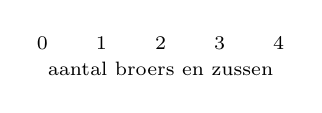
\begin{tikzpicture}[x=.75cm,y=.24cm,font=\scriptsize]
  \frequentieas{2}{12}{-.6}{4.6}
  \foreach \w/\f in {0/4,1/11,2/6,3/2,4/1}{\staaf{\w}{\f}{.55} \node[below] at (\w,0) {\w};}
  \node[below=9pt] at (2,0) {aantal broers en zussen};
\end{tikzpicture}}}

\begin{oefeningen}
\oef{h1-staaf}
\end{oefeningen}

\subsection{Het cirkeldiagram}

Wil je tonen welk deel van het geheel elke categorie is, dan kun je een cirkel verdelen in sectoren, zoals de stukken van een taart. Een volledige cirkel is $360^\circ$ en stelt alle gegevens voor. Een categorie met $25~\%$ van de gegevens krijgt dan een kwart van de cirkel: $90^\circ$.

\begin{theorie}
In een \textbf{\textcolor{accent}{cirkeldiagram}} krijgt elke categorie een sector met als middelpuntshoek

\vspace{1mm}
\qquad $\formule{\text{hoek} = \text{relatieve frequentie} \cdot 360^\circ}$
\end{theorie}

Een cirkeldiagram past alleen als de categorieën samen het geheel vormen, en als er weinig categorieën zijn. Verschillen tussen sectoren zie je minder goed dan verschillen tussen staven: gebruik het dus spaarzaam.

\voorbeeld{}{Van 40 leerlingen komen er 18 met de fiets, 12 met de bus, 6 te voet en 4 met de auto naar school. Teken een cirkeldiagram.\label{vb:h1-cirkel}}{%
\uitleg{We berekenen voor elke categorie de relatieve frequentie en vermenigvuldigen met $360^\circ$. De hoeken zijn samen $360^\circ$: dat is de controle.}
\naast{\begin{stappenvrij}{4.6cm}{4.4cm}
\text{fiets: } \tfrac{18}{40} \cdot 360^\circ = 162^\circ & $45~\%$ van de cirkel. \\
\text{bus: } \tfrac{12}{40} \cdot 360^\circ = 108^\circ & $30~\%$. \\
\text{te voet: } \tfrac{6}{40} \cdot 360^\circ = 54^\circ & $15~\%$. \\
\text{auto: } \tfrac{4}{40} \cdot 360^\circ = 36^\circ & $10~\%$. Samen $360^\circ$.
\end{stappenvrij}}{\begin{tikzpicture}[scale=1.15]
  \sector{90}{-72}{accent!55}{fiets}
  \sector{-72}{-180}{accent!35}{bus}
  \sector{-180}{-234}{accent!20}{te voet}
  \sector{-234}{-270}{accent!80}{\ auto}
\end{tikzpicture}}
Teken de sectoren met een geodriehoek, te beginnen bij een straal naar boven.}

\begin{oefeningen}
\oef{h1-cirkel}
\end{oefeningen}

\subsection{Het lijndiagram}

Hoe verandert iets in de loop van de tijd? Dan zet je de tijd op de horizontale as, een punt bij elke meting, en verbind je de punten. Zo zie je een stijging of daling meteen.

\begin{theorie}
Een \textbf{\textcolor{accent}{lijndiagram}} toont het verloop van een variabele in de tijd: punten bij de opeenvolgende tijdstippen, verbonden door lijnstukken.
\end{theorie}

De lijnstukken tussen de punten zijn geen metingen: ze helpen alleen het verloop te zien.

\voorbeeld{}{De schoolbibliotheek telt haar bezoekers per maand: september 310, oktober 285, november 260, december 190, januari 255, februari 240, maart 270, april 230, mei 180, juni 120. Teken een lijndiagram en beschrijf het verloop.\label{vb:h1-lijn}}{%
\uitleg{De maanden staan op de horizontale as, in de volgorde van het schooljaar. De verticale as gaat van 0 tot 350.}
\naast{\begin{minipage}[t]{5.6cm}\itshape Het aantal bezoekers daalt in de loop van het schooljaar. In december en in mei zakt het sterk: dan zijn er examens of vakanties. In januari en maart stijgt het weer even.\end{minipage}}{\begin{tikzpicture}[x=.85cm,y=.0085cm,font=\scriptsize]
  \frequentieas[bezoekers]{50}{350}{.4}{10.4}
  \foreach \m/\v [count=\i] in {sep/310,okt/285,nov/260,dec/190,jan/255,feb/240,maa/270,apr/230,mei/180,jun/120}{%
    \coordinate (p\i) at (\i,\v); \node[below,text height=1.5ex,text depth=.3ex] at (\i,0) {\m};}
  \draw[accent,thick] (p1) \foreach \i in {2,...,10}{-- (p\i)};
  \foreach \i in {1,...,10}{\fill[accent] (p\i) circle (2pt);}
\end{tikzpicture}}}

\begin{oefeningen}
\oef{h1-lijn}
\end{oefeningen}

\subsection{Het histogram}

Gegevens in klassen kun je niet voorstellen met losse staven: tussen de klassen $[50, 100[$ en $[100, 150[$ is geen opening, want een schermtijd van 99,5 minuten kan ook. Daarom laat je de staven op elkaar aansluiten.

\begin{theorie}
Een \textbf{\textcolor{accent}{histogram}} toont gegevens in klassen. Elke klasse krijgt een rechthoek met als basis de klasse en als hoogte de frequentie of de relatieve frequentie. De rechthoeken sluiten op elkaar aan.
\end{theorie}

Het verschil met een staafdiagram: de horizontale as van een histogram is een getallenas, met de klassengrenzen erop.

\voorbeeld{}{Teken een histogram van de schermtijden, met de klassen uit voorbeeld~\ref{vb:h1-klassen}.\label{vb:h1-histogram}}{%
\uitleg{De horizontale as is een getallenas van 50 tot 350 minuten, met een streepje bij elke klassengrens. De hoogte van elke rechthoek is de frequentie van de klasse.}
\figuren{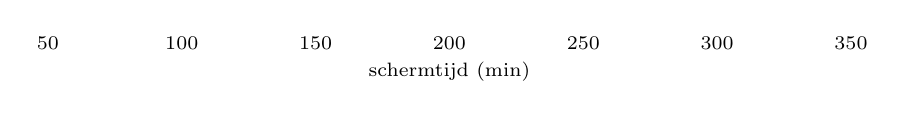
\begin{tikzpicture}[x=.034cm,y=.27cm,font=\scriptsize]
  \frequentieas{2}{12}{50}{356}
  \foreach \a/\f in {50/7,100/11,150/10,200/7,250/3,300/2}{\balk{\a}{\a+50}{\f}}
  \foreach \a in {50,100,...,350}{\node[below] at (\a,0) {\a};}
  \node[below=9pt] at (200,0) {schermtijd (min)};
\end{tikzpicture}}
Het histogram is hoog aan de linkerkant en loopt naar rechts langzaam af: de meeste leerlingen zitten één tot vier uur per dag op hun smartphone, enkelen veel langer.}

\begin{oefeningen}
\oef{h1-histogram}
\end{oefeningen}

\begin{alleenvoor}{2,3,4,5}
\subsection{Het stam-en-bladdiagram}

Een histogram toont de vorm, maar de precieze waarden zijn weg. Bij een kleine lijst kan het anders: je schrijft de getallen zelf in een tabel, gegroepeerd per tiental. Zo zie je de vorm én de waarden, en staan de gegevens meteen gerangschikt.

\begin{theorie}
In een \textbf{\textcolor{accent}{stam-en-bladdiagram}} splits je elk getal in een \textbf{\textcolor{accent}{stam}} (de tientallen) en een \textbf{\textcolor{accent}{blad}} (de eenheden). Elke stam staat één keer links, de bladen staan rechts ervan, van klein naar groot.
\end{theorie}

\voorbeeld{}{Twintig leerlingen halen deze scores op 100 voor een toets: 63, 81, 55, 72, 47, 68, 93, 75, 61, 70, 58, 84, 72, 66, 95, 52, 79, 63, 88, 77. Maak een stam-en-bladdiagram.\label{vb:h1-stamblad}}{%
\uitleg{De scores gaan van 47 tot 95: de stammen zijn 4 tot 9. We schrijven elk blad bij zijn stam, en ordenen daarna de bladen per rij.}
\naast{\begin{minipage}[t]{6.4cm}\itshape De regel $6 \mid 1\ 3\ 3\ 6\ 8$ betekent: 61, 63, 63, 66 en 68. Draai het diagram een kwartslag, en je ziet een staafdiagram: de meeste scores liggen tussen 60 en 80. Vermeld altijd wat de stam betekent, bijvoorbeeld $4 \mid 7 = 47$.\end{minipage}}{\renewcommand{\arraystretch}{1.15}\begin{tabular}{r|l}
4 & 7 \\ 5 & 2\ 5\ 8 \\ 6 & 1\ 3\ 3\ 6\ 8 \\ 7 & 0\ 2\ 2\ 5\ 7\ 9 \\ 8 & 1\ 4\ 8 \\ 9 & 3\ 5 \\[1mm]
\multicolumn{2}{l}{\scriptsize $4 \mid 7 = 47$}
\end{tabular}}}

\begin{oefeningen}
\oef{h1-stamblad}
\end{oefeningen}
\end{alleenvoor}

%========================================================================================
\section{De boxplot}

Hoe vat je een hele lijst samen in een paar getallen? Een idee: zet de gegevens van klein naar groot, en kijk welk getal in het midden staat. Dat getal verdeelt de gegevens in twee even grote groepen. Verdeel je elke groep nog eens in twee, dan heb je vier groepen met elk een kwart van de gegevens. Die grenzen tekenen we in een boxplot.

\subsection{De mediaan}

\begin{theorie}
De \textbf{\textcolor{accent}{mediaan}} $\formule{\Me}$ van een rij gegevens is het middelste getal als je de gegevens rangschikt van klein naar groot. Bij een even aantal gegevens is de mediaan het gemiddelde van de twee middelste getallen.
\end{theorie}

Bij $n$ gegevens staat de mediaan op plaats $\tfrac{n + 1}{2}$ in de gerangschikte rij. Bij $n = 9$ is dat plaats 5, bij $n = 10$ plaats 5,5: halfweg tussen het 5de en het 6de getal. Ongeveer de helft van de gegevens ligt onder de mediaan, de andere helft erboven.

\voorbeeld{}{Negen leerlingen tellen hoeveel berichten ze kregen tijdens de middagpauze: 12, 7, 15, 9, 4, 11, 9, 18, 6. Bepaal de mediaan.\label{vb:h1-mediaanoneven}}{%
\uitleg{Eerst rangschikken: de mediaan van een ongeordende lijst bestaat niet. Bij 9 getallen is er één middelste getal.}
\begin{stappen}
4,\ 6,\ 7,\ 9,\ \fbox{9},\ 11,\ 12,\ 15,\ 18 & Gerangschikt. Plaats $\tfrac{9 + 1}{2} = 5$. \\
\Me = 9 & Vier getallen links, vier rechts.
\end{stappen}}

\voorbeeld{}{Tien baby's wegen bij de geboorte (in kg): 3,2; 2,8; 3,9; 3,1; 2,5; 4,4; 3,6; 2,9; 3,3; 3,8. Bepaal de mediaan.\label{vb:h1-mediaaneven}}{%
\uitleg{Bij 10 getallen zijn er twee middelste getallen, op plaats 5 en 6. De mediaan ligt halfweg.}
\begin{stappenbreed}
2,5;\ 2,8;\ 2,9;\ 3,1;\ \fbox{3,2};\ \fbox{3,3};\ 3,6;\ 3,8;\ 3,9;\ 4,4 & Gerangschikt. Plaats $\tfrac{10 + 1}{2} = 5,5$. \\[1ex]
\Me = \dfrac{3,2 + 3,3}{2} = 3,25 \text{ kg} & Het gemiddelde van het 5de en het 6de getal.
\end{stappenbreed}
De mediaan hoeft dus geen waarde uit de lijst te zijn.}

\begin{oefeningen}
\oef{h1-mediaan}
\end{oefeningen}

\subsection{De kwartielen}

De mediaan verdeelt de gerangschikte gegevens in een onderste en een bovenste helft. Neem je van elke helft opnieuw de mediaan, dan krijg je twee nieuwe grenzen. Samen met de mediaan verdelen ze de gegevens in vier groepen van ongeveer een kwart. Er bestaan verschillende afspraken om die grenzen te berekenen. In dit boek gebruiken we deze.

\begin{theorie}
Rangschik de gegevens en splits ze in een onderste en een bovenste helft. Is het aantal gegevens oneven, dan hoort de mediaan bij geen van beide helften.
\begin{itemize}
  \item Het \textbf{\textcolor{accent}{eerste kwartiel}} $\formule{Q_1}$ is de mediaan van de onderste helft.
  \item Het \textbf{\textcolor{accent}{derde kwartiel}} $\formule{Q_3}$ is de mediaan van de bovenste helft.
\end{itemize}
\end{theorie}

De mediaan is dan het tweede kwartiel. Ongeveer een kwart van de gegevens ligt onder $Q_1$, en ongeveer een kwart boven $Q_3$. Je rekentoestel of een computerprogramma kan een andere afspraak gebruiken en dan een iets ander kwartiel geven, vooral bij weinig gegevens.

\voorbeeld{}{Elf leerlingen lossen een puzzel op. Hun tijden in seconden zijn: 34, 29, 41, 25, 38, 30, 45, 27, 36, 33, 52. Bepaal de mediaan en de kwartielen.\label{vb:h1-kwartielen}}{%
\uitleg{We rangschikken, zoeken de mediaan, en nemen dan de mediaan van de vijf getallen links en van de vijf getallen rechts. De mediaan zelf hoort bij geen van beide helften.}
\begin{stappenbreed}
\underbrace{25,\ 27,\ \fbox{29},\ 30,\ 33}_{\text{onderste helft}},\ \fbox{34},\ \underbrace{36,\ 38,\ \fbox{41},\ 45,\ 52}_{\text{bovenste helft}} & Elf getallen: de mediaan staat op plaats 6. \\
\Me = 34 & Het middelste getal. \\
Q_1 = 29 \qquad Q_3 = 41 & Het middelste getal van elke helft.
\end{stappenbreed}
Een kwart van de leerlingen heeft minder dan 29 seconden nodig, een kwart meer dan 41 seconden.}

\begin{werkwijze}
Rangschik de gegevens van klein naar groot. Zoek de mediaan. Splits de rij in twee helften (zonder de mediaan als het aantal oneven is), en zoek de mediaan van elke helft: dat zijn $Q_1$ en $Q_3$.
\end{werkwijze}

\begin{oefeningen}
\oef{h1-kwartielen}
\end{oefeningen}

\subsection{De boxplot tekenen}

Met de kleinste waarde, de kwartielen, de mediaan en de grootste waarde ken je de vijf grenzen van de vier groepen. Die vijf getallen teken je boven een getallenas.

\needspace{17\baselineskip}
\begin{theorie}
De \textbf{\textcolor{accent}{vijfgetallensamenvatting}} van een rij gegevens is: het minimum, $\formule{Q_1}$, $\formule{\Me}$, $\formule{Q_3}$ en het maximum.

\vspace{1mm}
In een \textbf{\textcolor{accent}{boxplot}} teken je boven een getallenas een rechthoek (de \textbf{\textcolor{accent}{box}}) van $Q_1$ tot $Q_3$, met een streep bij de mediaan. Twee lijnstukken (de \textbf{\textcolor{accent}{snorharen}}) gaan van de box naar het minimum en naar het maximum.

\figuren{\begin{tikzpicture}[x=1.1cm,font=\scriptsize]
  \boxplot[.7]{.7}{0}{2.5}{4}{6.5}{10}
  \draw[grijs] (0,0) -- (10,0);
  \foreach \x/\t in {0/minimum,2.5/$Q_1$,4/$\Me$,6.5/$Q_3$,10/maximum}{\draw[grijs] (\x,-.07) -- (\x,.07); \node[below] at (\x,-.07) {\t};}
  \foreach \a/\b in {0/2.5,2.5/4,4/6.5,6.5/10}{\node[above,text=grijs] at ({(\a+\b)/2},1.1) {25~\%};}
\end{tikzpicture}}
\end{theorie}

Elk van de vier stukken, de twee snorharen en de twee delen van de box, bevat ongeveer een kwart van de gegevens. Een kort stuk betekent dat de gegevens daar dicht bij elkaar liggen, een lang stuk dat ze ver uit elkaar liggen.

\voorbeeld{}{\alleenvoor{2,3,4,5}{Teken een boxplot van de twintig toetsscores uit voorbeeld~\ref{vb:h1-stamblad}.}\alleenvoor{1}{Twintig leerlingen halen deze scores op 100 voor een toets, al gerangschikt: 47, 52, 55, 58, 61, 63, 63, 66, 68, 70, 72, 72, 75, 77, 79, 81, 84, 88, 93, 95. Teken een boxplot.}\label{vb:h1-boxplot}}{%
\uitleg{\alleenvoor{2,3,4,5}{Het stam-en-bladdiagram geeft de scores al gerangschikt. }Bij 20 getallen bestaat elke helft uit 10 getallen.}
\begin{stappenbreed}
\text{min} = 47 \qquad \text{max} = 95 & Het eerste en het laatste getal. \\[1ex]
\Me = \dfrac{70 + 72}{2} = 71 & Het 10de en het 11de getal. \\[1.5ex]
Q_1 = \dfrac{61 + 63}{2} = 62 & Het 5de en het 6de getal van de onderste tien. \\[1.5ex]
Q_3 = \dfrac{79 + 81}{2} = 80 & Het 5de en het 6de getal van de bovenste tien.
\end{stappenbreed}
\figuren{\begin{tikzpicture}[x=.12cm,font=\scriptsize]
  \boxplot{.75}{47}{62}{71}{80}{95}
  \getalas[score]{40}{10}{100}
\end{tikzpicture}}}

\begin{werkwijze}
Bepaal de vijfgetallensamenvatting. Teken een getallenas met een gepaste schaal. Teken erboven de box van $Q_1$ tot $Q_3$, de streep bij de mediaan, en de snorharen tot het minimum en het maximum.
\end{werkwijze}

\begin{oefeningen}
\oef{h1-boxplot}
\end{oefeningen}

\subsection{Een boxplot lezen}

Een boxplot verbergt de afzonderlijke gegevens, maar zegt wel waar de kwarten liggen. Daarmee kun je uitspraken doen in procenten.

\voorbeeld{}{Terug naar het probleem. Een school vraagt aan 40 leerlingen van het 3de jaar hoeveel minuten ze gisteren op hun smartphone zaten. Dit zijn hun antwoorden.

\gegevens{|*{10}{c|}}{\hline
84 & 137 & 154 & 76 & 192 & 221 & 199 & 252 & 131 & 107 \\ \hline
75 & 66 & 110 & 232 & 118 & 162 & 141 & 155 & 200 & 238 \\ \hline
161 & 124 & 188 & 186 & 214 & 319 & 169 & 93 & 101 & 146 \\ \hline
269 & 305 & 58 & 76 & 218 & 173 & 103 & 245 & 286 & 139 \\ \hline}

Zitten de meeste leerlingen eerder één uur, twee uur of drie uur per dag op hun smartphone? Zit de helft van de leerlingen meer dan drie uur per dag op hun toestel? Teken een boxplot om het te beantwoorden.\label{vb:h1-terug}}{%
\uitleg{We rangschikken de 40 tijden. De onderste helft zijn de eerste 20, de bovenste helft de laatste 20.}
\begin{stappenbreed}
58,\ 66,\ 75,\ 76,\ 76,\ 84,\ 93,\ 101,\ 103,\ 107,\ 110,\ \dots,\ 305,\ 319 & Min 58, max 319. \\[1ex]
\Me = \dfrac{155 + 161}{2} = 158 & Het 20ste en het 21ste getal. \\[1.5ex]
Q_1 = \dfrac{107 + 110}{2} = 108,5 & Het 10de en het 11de getal. \\[1.5ex]
Q_3 = \dfrac{214 + 218}{2} = 216 & Het 30ste en het 31ste getal.
\end{stappenbreed}
\figuren{\begin{tikzpicture}[x=.042cm,font=\scriptsize]
  \boxplot{.75}{58}{108.5}{158}{216}{319}
  \draw[grijs,dashed] (180,0) -- (180,1.35) node[above] {3 uur};
  \getalas[min]{50}{50}{350}
\end{tikzpicture}}
Drie uur is 180 minuten. De mediaan is 158 minuten, minder dan drie uur: minder dan de helft van de leerlingen zit meer dan drie uur per dag op de smartphone. (Tel je na, dan zijn het er 16 van de 40.) Wel zit een kwart van de leerlingen meer dan 216 minuten op het toestel, dat is meer dan drie en een half uur. De middelste helft zit tussen 108,5 en 216 minuten op het toestel: ruwweg tussen twee uur en drie en een half uur, met de mediaan op ongeveer twee en een half uur. Het histogram (voorbeeld~\ref{vb:h1-histogram}) toont hetzelfde: de hoogste rechthoeken liggen tussen 100 en 200 minuten. De meeste leerlingen zitten dus tussen twee en drie uur per dag op hun smartphone: één uur is te weinig, en meer dan drie uur geldt maar voor een minderheid.}

\begin{werkwijze}
Een boxplot lezen: tussen twee opeenvolgende getallen van de vijfgetallensamenvatting ligt telkens ongeveer $25~\%$ van de gegevens. Onder de mediaan ligt dus ongeveer $50~\%$, onder $Q_3$ ongeveer $75~\%$.
\end{werkwijze}

\begin{oefeningen}
\oef{h1-lezen}
\end{oefeningen}

%========================================================================================
\opdrachtenkop

\begin{oefeningen}
\oef{h1-o1}

\needspace{12\baselineskip}
\oef{h1-o2}

\oef{h1-o3}

\oef{h1-o4}

\oef{h1-o5}

\oef{h1-o6}

\oef{h1-o7}

\needspace{12\baselineskip}
\oef{h1-o8}

\oef{h1-o9}

\oef{h1-o10}

\oef{h1-o11}

\oef{h1-o12}

\oef{h1-o13}

\needspace{12\baselineskip}
\oef{h1-o14}

\oef{h1-o15}

\oef{h1-o16}

\oef{h1-o17}

\oef{h1-o18}

\oef{h1-o19}

\oef{h1-o20}

\oef{h1-o21}

\oef{h1-o22}
\end{oefeningen}

%----------------------------------------------------------------------------------------
\opdrachtsectie{Test jezelf}

\begin{oefeningen}
\oef{h1-t1}

\oef{h1-t2}

\oef{h1-t3}

\oef{h1-t4}

\oef{h1-t5}

\oef{h1-t6}

\oef{h1-t7}
\end{oefeningen}

\herhaalschema{%
  \fv{oef:h1-t1}{vb:h1-soorten}{oef:h1-soorten}%
  \fv{oef:h1-t2}{vb:h1-tabel}{oef:h1-tabel}%
  \fv{oef:h1-t3}{vb:h1-cirkel}{oef:h1-cirkel}%
  \fv{oef:h1-t4}{vb:h1-histogram}{oef:h1-histogram}%
  \fv{oef:h1-t5}{vb:h1-kwartielen}{oef:h1-kwartielen}%
  \fv{oef:h1-t6}{vb:h1-boxplot}{oef:h1-boxplot}%
  \fv{oef:h1-t7}{vb:h1-terug}{oef:h1-lezen}}

\ifzelfstudie
\section*{Maak je eigen samenvatting}
Sluit dit boek en schrijf in je schrift: de soorten variabelen met een voorbeeld, wat frequentie, relatieve en cumulatieve frequentie betekenen, wanneer je een staafdiagram, cirkeldiagram, lijndiagram of histogram kiest, hoe je de mediaan en de kwartielen bepaalt, en hoe je een boxplot tekent en leest. Vergelijk daarna met de kaders.
\fi
